
\documentclass[journal]{IEEEtran}
\usepackage{blindtext}
\usepackage{listings}
\usepackage{color}
\usepackage{listings}
\usepackage{caption}
\usepackage{geometry}

\definecolor{dkgreen}{rgb}{0,0.6,0}
\definecolor{gray}{rgb}{0.5,0.5,0.5}
\definecolor{mauve}{rgb}{0.58,0,0.82}

\lstset{frame=tb,
  language=Java,
  aboveskip=3mm,
  belowskip=3mm,
  showstringspaces=false,
  columns=flexible,
  basicstyle={\small\ttfamily},
  numbers=none,
  numberstyle=\tiny\color{gray},
  keywordstyle=\color{blue},
  commentstyle=\color{dkgreen},
  stringstyle=\color{mauve},
  breaklines=true,
  breakatwhitespace=true,
  tabsize=3
}
\usepackage{graphicx}
\ifCLASSINFOpdf
  % \usepackage[pdftex]{graphicx}
  % declare the path(s) where your graphic files are
  % \graphicspath{{../pdf/}{../jpeg/}}
  % and their extensions so you won't have to specify these with
  % every instance of \includegraphics
  % \DeclareGraphicsExtensions{.pdf,.jpeg,.png}
\else
  % or other class option (dvipsone, dvipdf, if not using dvips). graphicx
  % will default to the driver specified in the system graphics.cfg if no
  % driver is specified.
  % \usepackage[dvips]{graphicx}
  % declare the path(s) where your graphic files are
  % \graphicspath{{../eps/}}
  % and their extensions so you won't have to specify these with
  % every instance of \includegraphics
  % \DeclareGraphicsExtensions{.eps}
\fi
\hyphenation{op-tical net-works semi-conduc-tor}


\begin{document}
%
% paper title
% can use linebreaks \\ within to get better formatting as desired
\title{Policy driven scaling of SaaS applications in hybrid clouds}
%
%
% author names and IEEE memberships
% note positions of commas and nonbreaking spaces ( ~ ) LaTeX will not break
% a structure at a ~ so this keeps an author's name from being broken across
% two lines.
% use \thanks{} to gain access to the first footnote area
% a separate \thanks must be used for each paragraph as LaTeX2e's \thanks
% was not built to handle multiple paragraphs
%

\author{Koen~Certyn,~\IEEEmembership{}
        supervisor: Bert~Lagaisse,~\IEEEmembership{Dr.,~KU Leuven,}
        promotor: ~Wouter~Joosen,~\IEEEmembership{Prof. dr. ir.,~KU Leuven}% <-this % stops a space
\thanks{M. Shell is with the Department
of Electrical and Computer Engineering, Georgia Institute of Technology, Atlanta,
GA, 30332 USA e-mail: (see http://www.michaelshell.org/contact.html).}% <-this % stops a space
\thanks{J. Doe and J. Doe are with Anonymous University.}% <-this % stops a space
\thanks{Manuscript received April 19, 2005; revised January 11, 2007.}}

% note the % following the last \IEEEmembership and also \thanks - 
% these prevent an unwanted space from occurring between the last author name
% and the end of the author line. i.e., if you had this:
% 
% \author{....lastname \thanks{...} \thanks{...} }
%                     ^------------^------------^----Do not want these spaces!
%
% a space would be appended to the last name and could cause every name on that
% line to be shifted left slightly. This is one of those "LaTeX things". For
% instance, "\textbf{A} \textbf{B}" will typeset as "A B" not "AB". To get
% "AB" then you have to do: "\textbf{A}\textbf{B}"
% \thanks is no different in this regard, so shield the last } of each \thanks
% that ends a line with a % and do not let a space in before the next \thanks.
% Spaces after \IEEEmembership other than the last one are OK (and needed) as
% you are supposed to have spaces between the names. For what it is worth,
% this is a minor point as most people would not even notice if the said evil
% space somehow managed to creep in.



% The paper headers
\markboth{Policy driven scaling of SaaS applications in hybrid clouds, Academic year 2014-2015}%
{Policy driven scaling of SaaS applications in hybrid clouds, Academic year 2014-2015}
% The only time the second header will appear is for the odd numbered pages
% after the title page when using the twoside option.
% 
% *** Note that you probably will NOT want to include the author's ***
% *** name in the headers of peer review papers.                   ***
% You can use \ifCLASSOPTIONpeerreview for conditional compilation here if
% you desire.




% If you want to put a publisher's ID mark on the page you can do it like
% this:
%\IEEEpubid{0000--0000/00\$00.00~\copyright~2007 IEEE}
% Remember, if you use this you must call \IEEEpubidadjcol in the second
% column for its text to clear the IEEEpubid mark.



% use for special paper notices
%\IEEEspecialpapernotice{(Invited Paper)}




% make the title area
\maketitle


\begin{abstract}
Most cloud application use private-or public cloud instances, but not both combined.
Both have their own benefits and downsides.
A hybrid cloud configuration uses both instances and combines them to reduce the downsides to a minimum while maximising the strengths of each platform.
Even though a hybrid cloud setup is very attractive, it is hard to configure.
This paper will provide a brief overview of the development of a middleware which offers, with the assistance of dynamic policies, SaaS applications the means to scale beyond their own limitations.
\end{abstract}
% IEEEtran.cls defaults to using nonbold math in the Abstract.
% This preserves the distinction between vectors and scalars. However,
% if the journal you are submitting to favors bold math in the abstract,
% then you can use LaTeX's standard command \boldmath at the very start
% of the abstract to achieve this. Many IEEE journals frown on math
% in the abstract anyway.

% Note that keywords are not normally used for peerreview papers.
\begin{IEEEkeywords}
Hybrid cloud, SaaS, Policy Driven, scaling.
\end{IEEEkeywords}

\IEEEpeerreviewmaketitle



\section{Introducion}
To stats, it's best to provide a short introduction in cloud computing, both basic and hybrid.
This will allow the reader to place this paper in a broader context.
\subsection{Cloud computing context}
The current state of computing has evolved enormously in the last ten years.
Systems were bound to their own power and limitations.
If these boundaries were crossed, additional hardware would be required.
With the arrival of public cloud computing, these limitations are history.
Unlimited resources are available, as long as you are willing to pay for it.\newline

In cloud computing, there are some different types of platforms available.
IaaS, PaaS and SaaS provide different platform types to suit every users' needs.\newline

The former platform, IaaS or Infrastructure as a Service, offers the possibility to create extremely adjustable virtual machines.
Administrators are able to configure the system completely how they see it.
This huge degree of flexibility goes hand in hand with the higher degree of complexity.\newline

Platform as a Service or PaaS providers will offer an already pre-configured server on which the user can run their own applications.
Even though they are still flexible, the degree of complexity is much lower compared to IaaS.
Basic dependencies (for example phpPgAdmin, Mongo, Jenkins, ..) can be installed without much trouble.

The latter platform type, SaaS or Software as a service is a platform which only offers a single type of application.
Mail and storage are typical examples of SaaS platforms.
The degree of flexibility is very low.

\begin{figure}[]
    \centering
    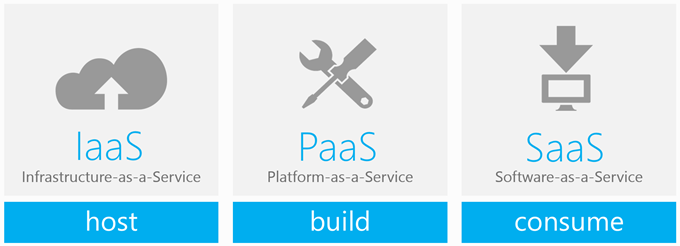
\includegraphics[width=\linewidth]{images/image2.png}
    \caption{Different types of cloudplatforms\cite{cloud_stack}}
    \label{fig:cloudplatforms}
\end{figure}

System administrators are offered the possibility to choose and use different types of platforms.
This will enable them to outsource some part of their system.
The benefits of this approach are huge.
System administrators will not be responsible to maintain the running servers, cloud providers will manage this.
Scalability will not pose a problem either.
Because of the scaling properties of cloudplatforms, the infrastructure will be able to follow the potential growth of the business.\newline

But ofcourse, there are downsides connected to the usage of cloudplatforms.
First of all, the possible vulnerability of private data.
Since only the providers have total control of the system, the ability to check what happens with the data is taken away.
Beside previously mentioned issue, the cost issue has to be addressed too.
Keeping up virtual machines is not cheap.
So costs will need to be monitored carefully.

\subsection{Hybrid cloud computing}
The hybrid cloud will offer a solution for these problems.
It will combine the benefits of a private cloudplatforms, on which the system administrator has total control, and the public cloudplatforms with unlimited scaling.
So hybrid cloud computing will present the best of both worlds: security, availability, scalability, limited costs and more control options.
Figure \ref{fig:hybridcloud} presents a global view of the interaction between both private and public cloud.


\begin{figure}[h!]
    \centering
    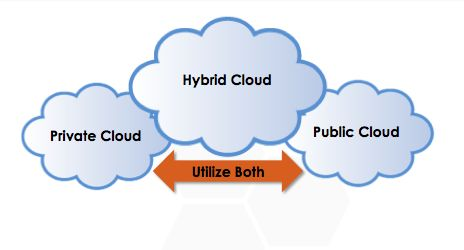
\includegraphics[width=\linewidth]{images/cloud_v_hybrid.jpg}
    \caption{Hybrid cloud computing\cite{IEEEhowto:kopka}}
    \label{fig:hybridcloud}
\end{figure}

\section{Problem statement and goals}\label{problems}
As already discussed in the introduction, the benefits of a hybrid cloud configuration are huge.
These benefits are very attractive to new smaller businesses but the implementation this setup is very complex.
This will cause them to hasitate to implement this very good feature.
The designed middleware will have to fulfil some problems that might arise.\newline

The major problem is the analysis of different types of data combined with the owners policies.
These policies will enable the system administrator to define carefully which actions will be taken after each event.
There are three different types of events.
First the monitoring of the private cloud.
This monitoring will trigger certain actions when critical values are exceeded.
These actions will mostly boot a new cloudplatform which can assist (temporary) with the load in the private cloud.
Secondly the analysis of entering requests.
Requests can be executed in both private and public cloud and contain custom properties.
These properties can vary in each application.
Again, these created requests will be compared to policies to achieve the proper reaction.\newline

It should be clear that the generation, creation and maintenance of these policies is the core aspect of the middleware.
Hence, the middleware has to achieve following goals;
\begin{itemize}
    \item Status control of the own private cloud.  In case critical values get crossed, actions should be taken.
    \item Different types of cloudplatforms must be support.
    \item The booting and termination of cloudplatforms.
    \item Sharing of load between different platforms.
    \item Changeable policies at runtime.
\end{itemize}

The complete evaluation will be done by :
\begin{itemize}
    \item The hybrid cloud configuration time.  This means the time it takes to implement the middleware on top of the current SaaS application.
    \item The difference in lines of code between a $"$brute force approach$"$ and the middleware to configure a hybride cloud setup.
    \item The actual benefit of the middleware.
\end{itemize}

\section{Used test Scenario's}\label{scenario}
To create an understandable context, two different types of SaaS applications are created.
These applications will be completely different to show the possible variability that the middleware and policies can provide.\newline

The basic start scenario is the same for both applications.
A starting entrepreneur wants to offer and develop a certain application.
To achieve this, he bought his own hardware to create a private cloud.
With a limited budget, he achieved to launch his own platform.
In the beginning the application has mediocre success.
The private cloud can perfectly manage all the incoming and exiting requests.
Everything seems fine in the first couple of months.
However, after some time, the application starts to gain an exponential growth of customers.
Customers are noticing more delays and unavailable services.
The entrepreneur is faced with a difficult decision.
He can take the risk and invest heavily in new hardware or he can choose to setup a hybrid cloud configuration.
So he chooses for the hybrid cloud configuration because he did not want to risk the heavy investment.
A hybrid cloud setup should be much cheaper.
The entrepreneur expects the support of the public cloud will be enough to relieve the pressure on the private cloud in difficult times.
Furthermore he expects the middleware to be configurable as he pleases.
As this is the basic context, the applications still need some description.\newline

The first application is storage based.
This application will focus on providing external storage support to customers.
Hard disk drives, to store data in the private cloud, will be a limiting factor.
Once these are full, no data can be stored anymore.
The hybrid cloud setup will offer a solution here.
If the local storage possibilities are getting limited, a public cloud is booted to assist with storing data.
This configuration will be able to scale nearly endlessly without having to buy additional HDD's.\newline

The second application is process based.
This application will focus on calculation based processes.
An information retrieval task is the perfect example.
Information retrieval tasks are very complex and can take up to multiple minutes to complete.
If a busy private cloud has to calculate a lot of these requests, delays will be notable.
Again, a public cloudplatform can aid with these calculations side by side the private cloudplatform.
This should enable the calculations to be executed much faster.
Every customer has its own degree of payment.
$"$Bronze$"$ users (eg. users that don't pay a lot) will be put on hold while premium users are given all means to speed up their calculations.\newline

\section{Contribution to state of the art}
The bases of the thesis is already constructed by \texttt{PaaShopper}\cite{PaaSHopper}.
\texttt{PaaSHopper} offers a middleware with the goal to offer organisations the possibility to manage their applications.
This managing is made possible by different policies which are defined in advance.
These offer guidance to all parts of the application and where they have to be executed in the hybrid cloud.
The \texttt{Policy-driven Execution Layer} is responsible for evaluation and execution of different policies including tenant specifications.
Besides that, an \texttt{Abstraction Layer} exists, which contains the core of the middleware.
This core contains the general management features and deployment facilities.\newline

Even though \texttt{PaaSHopper} offers a stable middleware, the policy system can be improved.
\texttt{PaaSHopper} uses static policies which are defined before compilation, so adjustments cannot be made at runtime.
The new middleware will offer a wider range of available policies which are adjustable at runtime.
This assures a much more flexible system.

Beside the adjustments to the policy system, an improvement of the cloud manage system was also required.
The use of public clouds comes with a certain cost (weekly, montly, ..).
Everyone wants to pay as least as possible, so keeping public instances online when they are not required means loss of own resources.
To counteract this, the newly designed middleware offers a \texttt{CloudManager} who keeps track of every public cloudplatform from start to finish.
By tracking the complete life cycle of public platform, no additional resources will be wasted.
Unused platforms will be terminated.

\section{Middleware development}
The middleware, able to solve the listed problems in section \ref{problems}, consists of two major parts; a \texttt{Policy Engine} component and a monitoring component.
SaaS providers who implement the middleware are offered multiple API's to interact with the system.
This section is structured as follows; to start the general idea behind the middleware is explained, secondly a more detailed explanation is provided that covers the \texttt{Policy Engine} which is the heart of the middleware and lastly the actual architecture is described.

\subsection{General idea behind the middleware}
An adjustable policy driven middleware will be provided to the SaaS provider.
Figure \ref{fig:general-middleware} gives a clearer view how the middleware will interact the existing system.\newline

The middleware is fully responsible to manage the scaling across both private and public cloud.
Existing systems will only see one endpoint and do not have to take any aspect of scaling into consideration.
They will be able to function as before.
However, when scaling across multiple platforms, rules have to be defined to manage these complex actions.
These rules will be converted in policies managed by the \texttt{Policy Engine}.

\begin{figure}[h!]
    \centering
    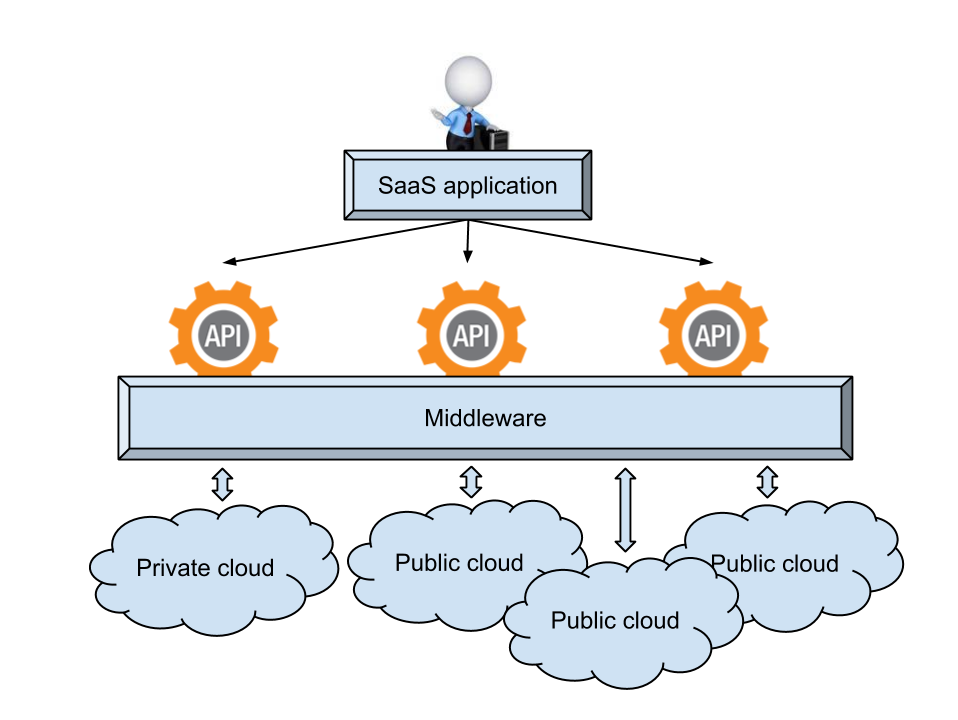
\includegraphics[width=\linewidth]{images/GeneralMiddleware.png}
    \caption{General middleware structure}
    \label{fig:general-middleware}
\end{figure}

To analyse the current situation in both private and public cloud, a \texttt{MonitorComponent} is created.
The first responsibility of this component is to track and monitor every change in the private cloud.
Doing this, the \texttt{MonitorComponent} is able to predict future problems and anticipate in advance.
Secondly the use of public clouds need to be tracked to assure no money is wasted by keeping unused public cloudplatforms up.\newline

Most of the components are ran inside the private cloud itself.
This choice was made because in public clouds, users do not have full control of the entire system.
Hence, the choice placing most of the complexity in the private cloud.
This approach however has some problems which are discussed in section \ref{discussion}.

\subsection{Policy Engine}
The policy engine consists of three major parts, each requiring their own set of rules.
First up, the monitoring policies who define rules and actions according to current measurements of the private clouds' critical points\footnote{The critical points can be amount of free memory left, used CPU, ..}.
Secondly cloud policies need to define rules to determine which cloudplatform should be booted for a specific job.
For example, it can't be that data that requires encryption is stored on a public cloudplatform that does not support encryption.
Lastly the request policies evaluate entering requests and determine if the action bound to the request should be executed in the private or public cloud.\newline

\subsubsection{Monitoring policies}
The goal of monitoring policies is to determine if a current value of the private cloud might be dangerous or not.
Dangerous, as in, might compromise the future performance of offered services.
If these dangerous states are detected early, action can be taken to assure services can run as smoothly even under heavy loads.
These actions will most of the time consist of booting new public cloudplatforms on which requests can be forwarded to.
This newly booted cloudplatform is only a backup, it will be discarded in case the situation in the private cloud improves.\newline

Basic provided policies in the middleware are :
\begin{itemize}
    \item When the amount of received requests is higher than a previously set benchmark, a new backup cloudinstance will be booted.
    \item If the load in the private cloud surpasses the value of 60\%, a new backup cloudinstance will be booted to assist the private cloud.
    \item In case the remaining free memory in the private cloud is less then 100MB, a new cloudinstance will be booted to assist with storing data.
\end{itemize}

The values defined in previous enumeration are default values which can be altered if desired.\newline

\subsubsection{Cloud policies}
When a cloudplatform is booted, a choice has to be made between the provided platforms.
To create a kind of comparison metric between platforms, a new XML based $"$language$"$ is introduced.
Listing \ref{lst:cloud} gives an configuration example of Heroku, a cloud provider. 
\begin{lstlisting}[caption=Cloud describing XML,label={lst:cloud}, frame=single]
<Cloud>
<Platform> Heroku </Platform>
<Encryption> Yes </Encryption>
<Log> Extended </Log>
<DataModel> Basic </DataModel>
<Processing> Basic </Processing>
<Deployment> Average </Deployment> 
<Cost> Low </Cost>
</Cloud>
\end{lstlisting}

The tags normally explain themselves.
\begin{itemize}
    \item Platform : Platform name
    \item Encryption : Is encryption provided or not?
    \item Log : Are actions logged, and how accurately?
    \item DataModel : Are there additional possibilities to store data? (eg. MongoDB, ..)
    \item Processing : The general processing power of the cloud;
    \item Deployment : How fast can a cloudinstance be booted from scratch?
    \item Cost : How much does maintaining this cloudinstance cost?
\end{itemize}
\subsubsection{Request policies}
The last type of policies are request policies which analyse incoming requests.
Basic request policies consist of very simple rules that do not take any additional priorities or properties into account.
For example: if the status of the private cloud is not overloaded (when requesting a certain calculation), this calculation will be executed in the private cloud.\newline

There are more advanced types of request policies, besides the basics'.
Property and priority request policies will keep track of additional information the request might offer.
For example: if a premium-user (= priority) wants to calculate something, but this cannot be done in the cloud (= property), all processes of not-premium users will be slowed down in the private cloud to guarantee fast calculation time to the premium user.
Another example : if a user wants to calculate something, but it has to be done quickly regardless of cost (= property), and the private cloud is fully overloaded, a cloud will have to be booted with fast deployment speed. 

\subsection{Middleware architecture}
The entire middleware is based on the principle of \texttt{Event-Condition-Action}.
An event will trigger the evaluation of this request which results in an action that will be taken.\newline

In the creation of the middleware, two different types of components are created.
Static components, the backbone of the middleware, are responsible of controlling and managing every action that will take place.  
These components will remain in the private cloud.
Next there are the hybrid components, which serve the actual calculation or storage application.
Hybrid components are able to run in both private and public cloud.
Figure \ref{fig:deployment-middleware} provides a better understanding of the interaction between components.

\begin{figure}[h!]
    \centering
    \includegraphics[width=\linewidth]{images/"General Deployment Diagram".png}
    \caption{General deployment structure}
    \label{fig:deployment-middleware}
\end{figure}
The components and their goals will be explained briefly.

\subsubsection{RequestChecker}
The \texttt{RequestChecker} is the first component every new request comes in contact with.
He will start the evaluation procedure and act according to the result.
\subsubsection{Cloudchecker}
The only task that the \texttt{CloudChecker} is to pick the perfect cloud for the given request.
To achieve the best result, the \texttt{CloudChecker} relies on the defined policies.
\subsubsection{CloudDeployer}
The name describes perfectly the use of this component.
This component is responsible to boot and terminate cloudinstances.
\subsubsection{CloudManager}
The \texttt{CloudManager} is responsible to check the availability and status of all booted cloudplatforms and to forward requests to the public cloud that have entered the private cloud.
\subsubsection{PrivateCloudMonitor}
The \texttt{PrivateCloudMonitor} is responsible to track the status of the own private cloud.
\subsubsection{PrivateCloudController}
The \texttt{PrivateCloudController} will be in charge of providing all status information about the own private cloud.
Besides that, he is responsible to initialise all applications in the private cloud itself.\newline

\section{Use of the middleware}
To integrate the middleware on top of a existing SaaS application, a few steps are required :
\begin{itemize}
    \item Integrate the full code of the middleware in the application;
    \item Adjust webserlvets and the \texttt{PrivateCloudController} to complete the link between both middleware and application;
    \item Select the backbone code of the application and place it into the $"$bootfolders$"$.  This code wil be deployed to the public cloud.
    \item (Optional) Add additional cloud platforms by providing meta information and a bootfile.
\end{itemize}

\section{Achieved Results}
After using the middleware to scale the scenario's presented in section \ref{scenario}, some results were obtained.\newline

The average time it takes to implement the middleware on top of the SaaS application is around one hour.
Take into consideration that these tests are done with very good knowledge of the system, so without this knowledge, it may consume a bit more time.\newline

After discussing the implementation time it might be good to give an in depth view of the effort (lines of code) that can be avoided by using the designed middleware.  
Tables \ref{tab:code1} and \ref{tab:code2} give a better comparison between both.

\captionof{table}{Middleware lines of code} \label{tab:code1} 
\begin{center}
\begin{tabular}{ |l|l| } \hline \multicolumn{2}{|c|}{Middleware lines of code} \\
\hline
PolicyEngine & \textasciitilde450\\
Controllers & \textasciitilde250\\
Monitors & \textasciitilde275\\
Entiteiten & \textasciitilde460\\\hline
Servlet Adjustments & \textasciitilde30\\
PrivateCloudController & \textasciitilde50\\
\hline 
\end{tabular}
\end{center}

\captionof{table}{Required lines of code without middleware} \label{tab:code2} 
\begin{center}
\begin{tabular}{ |l|l| } \hline \multicolumn{2}{|c|}{Required lines of code without middleware} \\
\hline
Policies & \textasciitilde600\\
Other requirements & \textasciitilde1000\\
\hline 
\end{tabular}
\end{center}

In the comparison, a difference of \textasciitilde1500 lines of code is noticeable.  When using the middleware, only the servlet adjustments and \texttt{PrivateCloudController} need to be adjustsed.

Lastly the comparison in request answer times.

\begin{center}
\begin{tabular}{ |l|l|l| } \hline Load & Private & Public \\
\hline
Low & \textasciitilde50 & \textasciitilde45\\
Low & \textasciitilde80 & \textasciitilde45\\
Low & \textasciitilde120 & \textasciitilde45\\
\hline 
\end{tabular}
\end{center}
\captionof{table}{Comparison in average response time} \label{tab:code3} 

Tabular \ref{tab:code3} offers a clearer view of the benefits that can be accomplished while using the designed middleware.
However, when a new public cloud instance has to be booted, a loss of \textasciitilde180 has to be taken into consideration.
Hence the reason the monitoring aspect is so crucial.

\section{Future work and discussion points}\label{discussion}
The suggested middleware has different strong and weak points.
Weaker points allow possible refinement in future work.\newline

First, the ease of integration is a big plus.  
This causes a very low entry-point at which SaaS providers might be willing to implement the middleware.
Secondly the adjustable policies offer the users of the middleware full control over the actions of the middleware, even at-runtime.\newline

The \texttt{Policy Engine}, which is the heart of the middleware runs on a single instance in the private cloud.
This creates a single point of failure which can be fatal in certain applications.
The same is true concerning the entities keeping track of booted cloudplatforms.  
A hardware crash resulting in loss of data will cause any information of booted clouds will be lost.
This is possible to avoid using data and process replication between multiple servers in the private cloud.

\section{Conclusion}
The designed middleware is able to offer a simple way of integration on top of an existing SaaS application to create a bridge between both private and public clouds, a hybrid cloud setup.
This enables the SaaS application to scale beyond own resources, provided in the own private cloud.
Furthermore, the user implementing the middleware is able to configure all policies himself and add addition public cloud platforms if needed, so complete control is guaranteed.





% if have a single appendix:
%\appendix[Proof of the Zonklar Equations]
% or
%\appendix  % for no appendix heading
% do not use \section anymore after \appendix, only \section*
% is possibly needed

% use appendices with more than one appendix
% then use \section to start each appendix
% you must declare a \section before using any
% \subsection or using \label (\appendices by itself
% starts a section numbered zero.)
%



% Can use something like this to put references on a page
% by themselves when using endfloat and the captionsoff option.
\ifCLASSOPTIONcaptionsoff
  \newpage
\fi



% trigger a \newpage just before the given reference
% number - used to balance the columns on the last page
% adjust value as needed - may need to be readjusted if
% the document is modified later
%\IEEEtriggeratref{8}
% The "triggered" command can be changed if desired:
%\IEEEtriggercmd{\enlargethispage{-5in}}

% references section

% can use a bibliography generated by BibTeX as a .bbl file
% BibTeX documentation can be easily obtained at:
% http://www.ctan.org/tex-archive/biblio/bibtex/contrib/doc/
% The IEEEtran BibTeX style support page is at:
% http://www.michaelshell.org/tex/ieeetran/bibtex/
%\bibliographystyle{IEEEtran}
% argument is your BibTeX string definitions and bibliography database(s)
%\bibliography{IEEEabrv,../bib/paper}
%
% <OR> manually copy in the resultant .bbl file
% set second argument of \begin to the number of references
% (used to reserve space for the reference number labels box)
\begin{thebibliography}{1}

\bibitem{IEEEhowto:kopka}
H.~Kopka and P.~W. Daly, \emph{A Guide to \LaTeX}, 3rd~ed.\hskip 1em plus
  0.5em minus 0.4em\relax Harlow, England: Addison-Wesley, 1999.

\end{thebibliography}

% biography section
% 
% If you have an EPS/PDF photo (graphicx package needed) extra braces are
% needed around the contents of the optional argument to biography to prevent
% the LaTeX parser from getting confused when it sees the complicated
% \includegraphics command within an optional argument. (You could create
% your own custom macro containing the \includegraphics command to make things
% simpler here.)
%\begin{biography}[{\includegraphics[width=1in,height=1.25in,clip,keepaspectratio]{mshell}}]{Michael Shell}
% or if you just want to reserve a space for a photo:

% You can push biographies down or up by placing
% a \vfill before or after them. The appropriate
% use of \vfill depends on what kind of text is
% on the last page and whether or not the columns
% are being equalized.

%\vfill

% Can be used to pull up biographies so that the bottom of the last one
% is flush with the other column.
%\enlargethispage{-5in}



% that's all folks
\end{document}


